%%%%%%%%%%%%%%%%%%%%%%%%%%%%%%%%%%%%%%%%%%%%%%%%%%%%%%%%%%%%%%%
%
% Welcome to Overleaf --- just edit your LaTeX on the left,
% and we'll compile it for you on the right. If you open the
% 'Share' menu, you can invite other users to edit at the same
% time. See www.overleaf.com/learn for more info. Enjoy!
%
%%%%%%%%%%%%%%%%%%%%%%%%%%%%%%%%%%%%%%%%%%%%%%%%%%%%%%%%%%%%%%%
\documentclass[a4paper, 12pt]{my_cv}
\usepackage[margin=0mm]{geometry}
\usepackage{tgheros}
\usepackage{tikz}
\usetikzlibrary{fit,calc}
\usepackage{graphicx,wrapfig}
\graphicspath{ {./images/} }
\usepackage{svg}
\svgpath{ {./images/} }
\usepackage{textpos}
\setlength{\unitlength}{1mm}
\usepackage{everypage}
\usepackage{setspace}
\usepackage{lipsum}
\usepackage{tabu}
\usepackage{hyperref}
\usepackage{dcolumn}


\newlength\MyColWidth
\setlength\MyColWidth{70mm}
\newlength\TopBarHeight
\setlength\TopBarHeight{60mm}
\newlength\MyTopMargin
\setlength\MyTopMargin{12mm}
\newlength\MyLeftMargin
\setlength\MyLeftMargin{5mm}
\newlength\MyRightMargin
\setlength\MyRightMargin{5mm}
\newlength\MainWidth
\setlength\MainWidth{\dimexpr\paperwidth-\MyColWidth-\MyRightMargin}
\newlength\SideWidth
\setlength\SideWidth{\dimexpr\MyColWidth-\MyLeftMargin}
\parindent7mm
\definecolor{Leaf}{HTML}{656d29}
\definecolor{Stem}{HTML}{a8a660}
\definecolor{Aloe}{HTML}{dadfbc}
\definecolor{Petal}{HTML}{e8f1f8}
\definecolor{MyDandelion}{HTML}{e88e01}
\pagecolor{Petal}

\AddEverypageHook{%
\begin{tikzpicture}[overlay, remember picture]
        \definecolor{Leaf}{HTML}{656d29}
        \definecolor{Stem}{HTML}{a8a660}
        \definecolor{Aloe}{HTML}{dadfbc}
        \definecolor{Petal}{HTML}{e8f1f8}
        \definecolor{MyDandelion}{HTML}{e88e01}
        # Define a Tikz Path with reference point at current page north west, moving its reference point by (+horoffset, -veroffset). from this path, define a node with the characteristics in the square brackets
        \path (current page.north west) ++(\hoffset, -\voffset) node[anchor=north west, shape=rectangle, inner sep=0, minimum width=\paperwidth, minimum height=\paperheight] (pagearea) {};
        # Now define a path that starts at the NW point of previous node, offset it by
        \path (pagearea.north west) ++(+\currentsidemargin,-\topmargin-\headheight-\headsep) node[anchor=north west, shape=rectangle, inner sep=0, minimum width=\textwidth, minimum height=\textheight] (textarea) {};
        \path (pagearea.north west) ++(\hoffset, -\voffset) node[anchor=north west, shape=rectangle, inner sep=0, minimum width=\MyColWidth, minimum height=\paperheight] (marginbox) {};
        \draw[fill=Aloe,Aloe] (marginbox.north west) rectangle (marginbox.south east);
    \end{tikzpicture}
}

\begin{document}\fontfamily{qhv}\selectfont
\TPMargin{2mm}
\begin{textblock*}{\SideWidth}(\MyLeftMargin,0.5\MyTopMargin)
    \centering
    % \includegraphics[width = \textwidth]{images/qrcode.eps}
    \begin{figure}[t]
    
\includegraphics[height = 40mm]{images/portrait_round.png}
    \end{figure}

    \section{Contacts}

    \begin{table}[t]
            \centering
            \begin{tabular*}{0.95\MyColWidth}{>{\raggedleft}p{0.2\MyColWidth}|l}
                \includesvg[height = 1em]{Smartphone}   & \href{tel:+393408000465}{+39 3408000465} \\ [.2em]
                \includesvg[width = 1em]{mail}          & \href{mailto:marco3bissaro@gmail.com}{marco3bissaro@gmail.com} \\ [.2em]
                
\includegraphics[height = 1em]{images/GitHub-cropped.png} & \href{https://github.com/MSnaker}{github.com/MSnaker}\\ [.2em]
                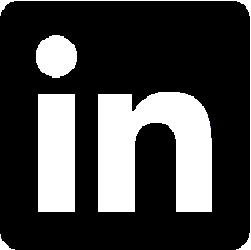
\includegraphics[height = 1em]{images/LinkedIn-cropped.png} & \href{https://www.linkedin.com/in/m-bissaro/}{linkedin.com/in/m-bissaro} \\ [.2em]
                
\includegraphics[height = 1em]{images/goodreads_icon_100x100.png} & \href{https://www.goodreads.com/drsnek}{goodreads.com/drsnek}
            \end{tabular*}
    \end{table}

    \section{Languages}
    
    \begin{table}[t]
        \begin{tabular*}{0.95\MyColWidth}{>{\raggedleft}p{0.2\MyColWidth}|l}
             Italian &  Native\\ 
             English &  Expert\\ 
             German  &  Elementary
        \end{tabular*}
    \end{table}

    \section{Education}
    {\raggedright
    \datedsubsection{MSc. Aerospace Engineering}{\newline2017-2020}
    University of Padua,\newline Erasmus Student at RWTH Aachen.

    \datedsubsection{BSc. Aerospace Engineering}{\newline2014-2017}
    \raggedright University of Padua.
    
    }

\section{Technical Skills}
    \begin{table}[t]
        \begin{tabular*}{0.95\MyColWidth}{>{\raggedleft}p{0.2\MyColWidth}|l}
              & Python\\ 
              & Matlab \& Simulink\\ 
              & Git\\ 
              & Linux\\
              & Office Suite\\
        \end{tabular*}
    \end{table}

    \section{Soft Skills}
    \begin{table}[t]
        \begin{tabular*}{0.95\MyColWidth}{>{\raggedleft}p{0.2\MyColWidth}|l}
              & Critical Thinking\\ 
              & Problem Solving\\
              & Stress Resilience\\
              & Teamwork
        \end{tabular*}
    \end{table}

    \section{Volunteering}
    Blood donor since 2013
\end{textblock*}

\TPMargin{5mm}
\begin{textblock*}{\MainWidth}(\MyColWidth,0.8\MyTopMargin){
    % \renewcommand{\baselinestretch}{1.5}
    \centering{\name{Marco}{Bissaro}}
    
    \centering{\jobtitle{Aerospace Engineer}}
    
    
    % {\small Death\newline \normalsize begets Death\newline \large begets Death...}
    % {and time\newline Shall gurgle on...}
    % {“a jack of all trades is a master of none, but oftentimes better than a master of one”}
    % \textit{Stand out, \\don't blend in.}
    % \textit{Show intelligence,\\ not cleverness.}
    }
        
    \section{About me}
      AIV Software Engineer with a Master's Degree in Aerospace Engineering from University of Padua and international experience at RWTH Aachen. Possessing a solid grasp on physical phenomena, I excel at both direct problem-solving and methodical evisceration of complex challenges. My experience forged me to obtain consistent results and I give my best in a collaborative team. I strive for continuous learning, and that means I am in a perpetual journey of improvement—sometimes learning something new, sometimes honing my current skills.

    \section{Work Experience}
    \datedsubsection{D-Orbit}{2022 - }
    \begin{itemize}
        \item \datedsubsection{AIV Software Engineer}{2022 - }
    
    The role is mainly dedicated to the development of scripts to automate the Spacecraft AIV procedures, however, the required knowledge of the S/C software and hardware is also applied in providing support during the AIV phases.
    
        \item \datedsubsection{Flight Software Engineer}{2024 - 2025}
    
    The role's purpose is to develop Flight Software routines for the Spacecraft's Mode Control, Thermal Control, and FDIR (Fault Detection, Isolation, and Recovery) mechanisms. This development process encompasses software requirements definition, flow design, and code writing. These routines are written in MicroPython and interface with the operating system through both built-in and company-specific modules.
    \end{itemize}
    
          
    \datedsubsection{Zanardi Fonderie}{2021 - 2022}
    \begin{itemize}
        \item \datedsubsection{Technical Area Engineer}{2021 - 2022}

    The role was dedicated to developing and maintaining Technical specifications for the machining department.

        \item \datedsubsection{Automotive Certification Engineer}{2021 - 2022}

    The role was focused on the evolution of the company towards compliance with the IATF 16949 (Automotive) norm.
    \end{itemize}

    \section{Personal Projects}

    \datedsubsection{Python Password Generator}{2021}
    
    Python script with GUI to obtain a password from a previously encrypted source text. The script is meant to adopt an algorithm easy to replicate mentally with the correct source on hand, so that it is not essential to have the tool at hand, to obtain a password.

    \datedsubsection{PC tower shelf}{2021}
    
    Sheet metal design of a custom shelf for my Personal Computer. The shelf adapted to the desk structure, and was supported at its free edge by two steel cables, which also kept the PC tower from oscillating.
    
\end{textblock*}


\end{document}
